% 
% topic Template for ME3023 - Measurements in Mechanincal Systems - Tennessee Technological University
%
% Spring 2020 - Summer 2020
% Tristan Hill, May 31, 2020
% Demonstration 1 - Dimensional Instruments
% Topic 2 - Using Calipers 
%

\documentclass{beamer}                         % for presentation (has nav buttons at bottom)
%\documentclass[handout]{beamer}  % for handout 
\usepackage{beamerthemesplit}
\usepackage{amsmath}
\usepackage{listings}
\usepackage{multicol}
\usepackage{framed}

\beamertemplateballitem

\definecolor{TTUpurple}{rgb}{0.3098, 0.1607, 0.5176} % TTU Purple (primary)
\definecolor{TTUgold}{rgb}{1.0000, 0.8666, 0.0000} % TTU Gold (primary)

\setbeamercolor{palette primary}{bg=TTUpurple,fg=TTUgold}
\setbeamercolor{palette secondary}{bg=black,fg=TTUgold}
\setbeamercolor{palette tertiary}{bg=black,fg=TTUpurple}
\setbeamercolor{palette quaternary}{bg=TTUgold,fg=black}
\setbeamercolor{structure}{fg=TTUpurple} % itemize, enumerate, etc
\setbeamercolor{section in toc}{fg=TTUpurple} % TOC sections

% custom colors 
\definecolor{mygray}{rgb}{.6, .6, .6}
\definecolor{mypurple}{rgb}{0.6,0.1961,0.8}
\definecolor{mybrown}{rgb}{0.5451,0.2706,0.0745}
\definecolor{mygreen}{rgb}{0, .39, 0}
\definecolor{mypink}{rgb}{0.9960, 0, 0.9960}

% color commands
\newcommand{\R}{\color{red}}
\newcommand{\B}{\color{blue}}
\newcommand{\BR}{\color{mybrown}}
\newcommand{\K}{\color{black}}
\newcommand{\G}{\color{mygreen}}
\newcommand{\PR}{\color{mypurple}}
\newcommand{\PN}{\color{mypink}}
\newcommand{\GD}{\color{TTUgold}}
\newcommand{\OR}{\color{orange}}

\newcommand{\Lagr}{\mathcal{L}} % lagrangian

\newcommand{\vspccc}{\vspace{6mm}\\} % large vertical space
\newcommand{\vspcc}{\vspace{4mm}\\}   % medium vertical space
\newcommand{\vspc}{\vspace{2mm}\\}     % small vertical space

\newcommand{\hspcccc}{\hspace{10mm}} % large horizontal space
\newcommand{\hspccc}{\hspace{6mm}} % large horizontal space
\newcommand{\hspcc}{\hspace{4mm}}   % medium horizontal space
\newcommand{\hspc}{\hspace{2mm}}     % small horizontal space


\author{ME3023 - Measurements in Mechanical Systems} % original formatting from Mike Renfro, September 21, 2004

\newcommand{\DNUM}{1\hspace{2mm}} % Demonstration number
\newcommand{\TNUM}{2\hspace{2mm}} % Topic number  
\newcommand{\demotitle}{Dimensional Instruments }
\newcommand{\topictitle}{Using A Micrometer} 

\newcommand{\sectiontitleI}{Overview}
\newcommand{\sectiontitleII}{Components}
\newcommand{\sectiontitleIII}{Vernier Micrometer}
\newcommand{\sectiontitleIV}{Digital Micrometer}

\title{Demonstration \DNUM - \demotitle}

\date{Mechanical Engineering\vspc Tennessee Technological University}

\begin{document}

\lstset{language=MATLAB,basicstyle=\ttfamily\small,showstringspaces=false}

\frame{\titlepage \center\begin{framed}\Large \textbf{Topic \TNUM - \topictitle}\end{framed} \vspace{5mm}}

% Section 0: Outline
\frame{

\large \textbf{Topic \TNUM - \topictitle} \vspace{3mm}\\

\begin{itemize}
	\item \sectiontitleI		\vspc % Section I
	\item \sectiontitleII 	\vspc % Section II
	\item \sectiontitleIII 	\vspc %Section III
	\item \sectiontitleIV 	\vspc %Section IV
\end{itemize}

}

% Section I:
\section{\sectiontitleI}

\frame{
\frametitle{\sectiontitleI}

A micrometer, sometimes known as a micrometer screw gauge, is a device incorporating a calibrated screw widely used for accurate measurement of components[1] in mechanical engineering and machining as well as most mechanical trades, along with other metrological instruments such as dial, vernier, and digital calipers. {\tiny Text: \href{https://en.wikipedia.org/wiki/Micrometer}{Wikipedia}}\vspc

Unlike a pair of Vernier or digital calipers, most micrometers are designed to measure outside dimensions only. \vspc

{\tiny Text: \underline{Theory and Design of Mechanical Measurements, 5th Edition}}
}


% Section II:
\section{\sectiontitleII}

\frame{
\frametitle{\sectiontitleII}

        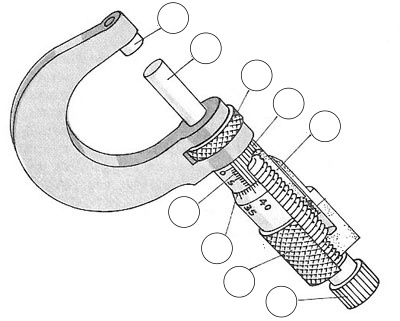
\includegraphics[scale=.35]{micrometer_fig2.png}
        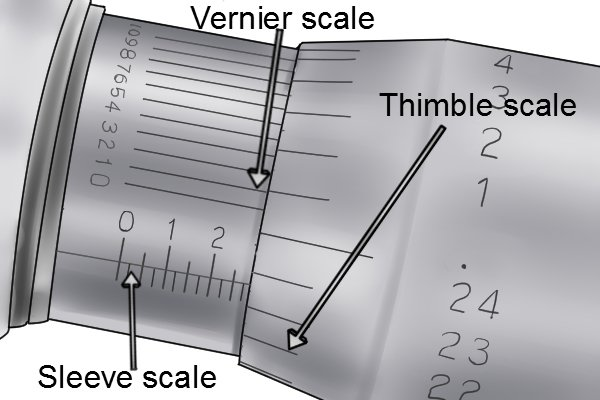
\includegraphics[scale=.25]{micrometer_fig1.png}
        \begin{multicols}{2}
        	\begin{enumerate}
 			\item Anvil
 			\item Spindle
 			\item Thimble
 			\item Lock Ring
 			\item Sleeve Scale
 			\item Thimble Scale
 			\item Vernier Scale
 			\item Ratchet (Clutch) Knob			
 		\end{enumerate}
 		\end{multicols}

}



% Section III:
\section{\sectiontitleIII}

\frame{
\frametitle{\sectiontitleIII}

A vernier scale is a visual aid to take an accurate measurement reading between two graduation markings on a linear scale by using mechanical interpolation; thereby increasing resolution and reducing measurement uncertainty by using Vernier acuity to reduce human estimation error.  {\tiny \href{https://en.wikipedia.org/wiki/Vernier_scale}{Wikipedia}}

\begin{multicols}{2}
\underline{Pros}
\begin{itemize}
\item 
\item
\item
\end{itemize}
\underline{Cons}
\begin{itemize}
\item 
\item
\item
\end{itemize}
\end{multicols}

}

\frame{
\frametitle{\sectiontitleIII}

Look at scale carefully and clean the jaws before you take a measurement. First look at the main scale then add the measurement from the Vernier scale. \vspace{40mm}\\

}


% Section IV:
\section{\sectiontitleIV}

\frame{
\frametitle{\sectiontitleIV}

A digital micrometer contains an embedded processor and user interface to facilitate the measurement process.

\begin{multicols}{2}
\underline{Pros}
\begin{itemize}
\item 
\item
\item
\end{itemize}
\underline{Cons}
\begin{itemize}
\item 
\item
\item
\end{itemize}
\end{multicols}

}

\frame{
\frametitle{\sectiontitleIV}

Make sure to clean the jaws and zero the instrument before you take a measurement. Also, be careful not to press the zero button on accident. On some models this is very easy to do. \vspace{40mm}\\

}


\end{document}





